\documentclass[12pt]{article}
\usepackage{geometry}                % See geometry.pdf to learn the layout options. There are lots.
\geometry{letterpaper}                   % ... or a4paper or a5paper or ... 
%\geometry{landscape}                % Activate for for rotated page geometry
%\usepackage[parfill]{parskip}    % Activate to begin paragraphs with an empty line rather than an indent
\usepackage{graphicx}
\usepackage{amssymb}
\usepackage{subfig}
\usepackage{multirow}
\usepackage[margin=20pt, font=small,labelfont=sc, labelsep=endash]{caption}
\usepackage{pstricks, pst-node,pst-tree}


\title{Analysis of loadings}
\author{Wesley Brooks}
\date{}                                           % Activate to display a given date or no date

\usepackage{Sweave}
\begin{document}
\setkeys{Gin}{width=0.9\textwidth}    %make figures a bit wider than the Sweave default.
\maketitle























\begin{figure}[h!]
    \begin{center}
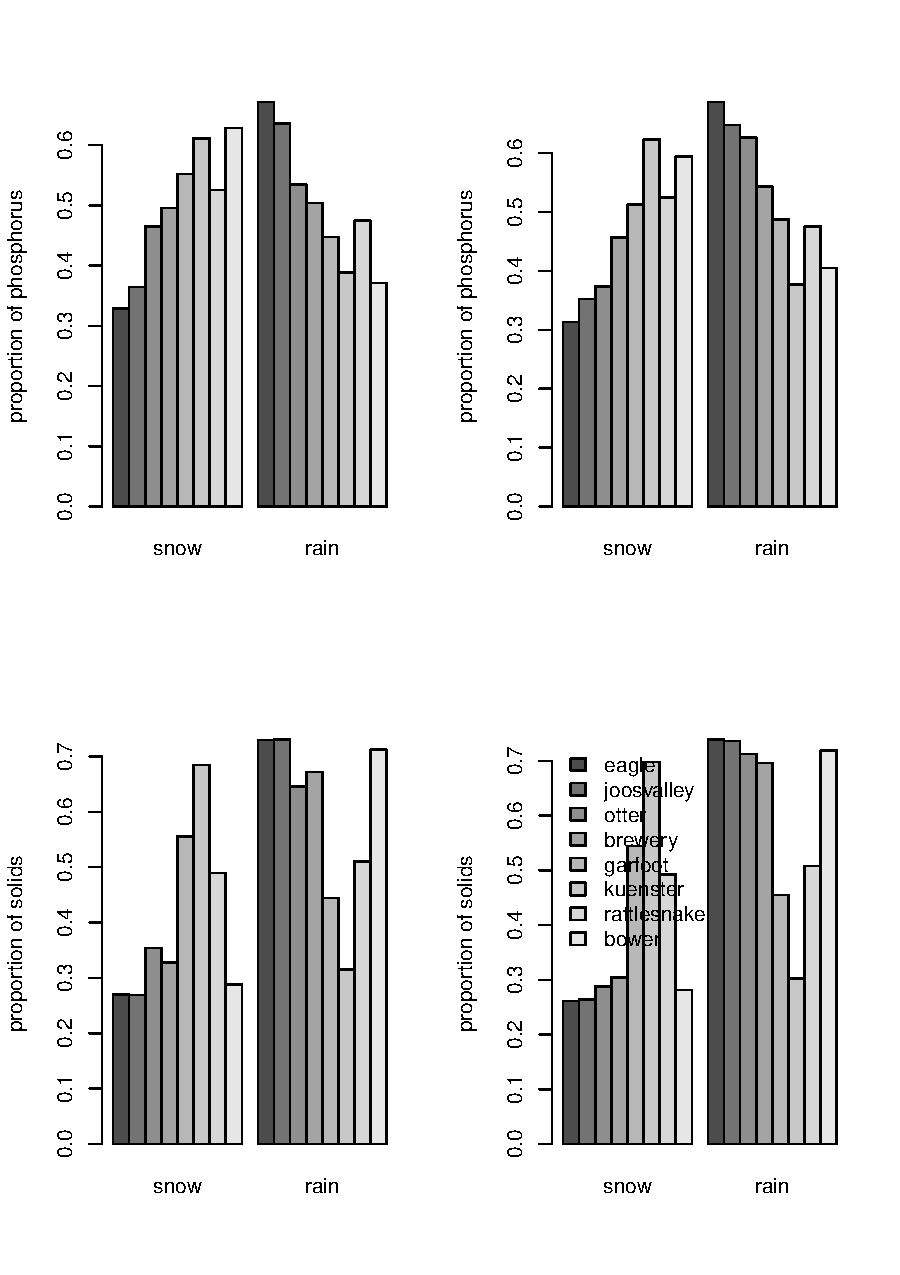
\includegraphics{loadings-fig2}
    \end{center}
    \vspace{-10mm}
    \caption{Cumulative storm loadings at the four creeks.\label{bars}}
\end{figure}












%Boxplots of the contribution from individual storm events
\begin{figure}[h]
    \setkeys{Gin}{width=1\textwidth}    %make figures a bit wider than the Sweave default.
    \begin{center}
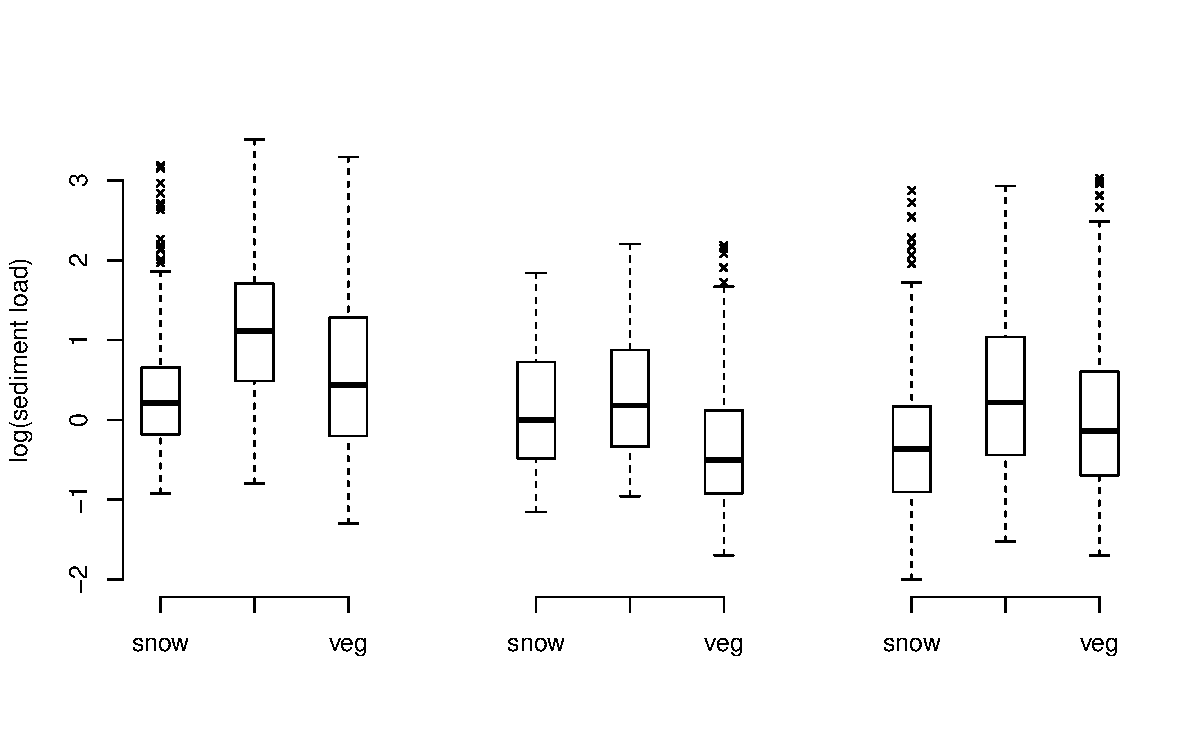
\includegraphics{loadings-boxplot_stot}
    \vspace{15mm}
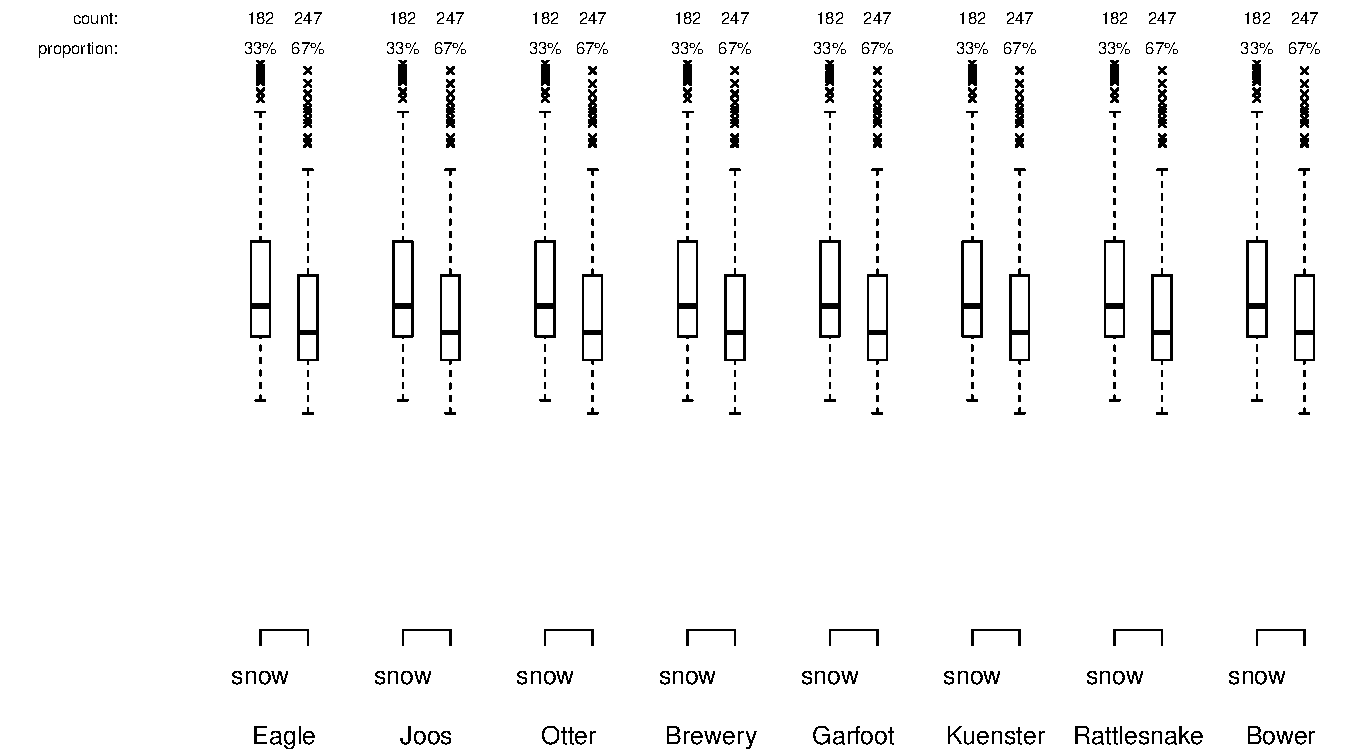
\includegraphics{loadings-boxplot_ptot}
    \caption{Boxplots showing the sediment and phosphorus load produced by individual events at all four streams.\label{boxplots}}
    \end{center}
\end{figure}


















\section{Data}

\paragraph{Description}
The data in this report comes from four Wisconsin streams that were monitored (with some gaps in data collection) between 1989 and 2007. The streams and the period during which each was monitored are:

\begin{table}[h]
\begin{center}
\begin{tabular}{r c l}
        \textbf{Stream}  & \textbf{Events} & \textbf{Years}\\
        Eagle & 429 &1991-1994, 2003-2007\\
        Joos Valley & 473 & 1990-1994, 2002-2007\\
        Otter & 424 & 1990-1997, 2000-2002\\
        Brewery & 670 & 1989, 1994-2002, 2004-2005\\
        Garfoot & 527 & 1985, 1990-1993, 1995-1998\\
        Kuenster & 218 & 1992-1995\\
        Rattlesnake & 170 & 1991-1994\\
        Bower & 373 & 1990-1994, 2006-2009\\
    \end{tabular}
\end{center}
\end{table}

Each entry in our data set represents one loading event, which is defined based on the hydrograph - the event begins when the loading rises from a base level toward a peak, and ends when the loading falls back to its new base level. Two kinds of load are measured for each event - the sediment load and the phosphorus load. There are two typical ways that sediment and phosphorus get into streams - they can be carried either by runoff during a rainstorm or by melting snow.\\

Not all of the data can be collected for each event. For instance, rainfall is measured only when the ground is free of snow because snow interferes with the rain gauges. And the amount of snowmelt is estimated by multiplying the water content of the snow by the change in snow depth a warm snap, which is inaccurate when additional snow falls during that event. Broadly, there is one set of measurements that are made during rainfall-driven events and a different set of measurements that are made during snowmelt-driven events. Because of this, the two types of event are modeled separately.\\

\paragraph{Exploratory Analysis}
Our anaysis targets the phosphorus and sediment loads carried by each stream. Using Rainmaker software, each load can be broken into two parts: base load and storm load. We will consider models of the storm load and of the total load.\\

The first task was to decide whether most of the annual load is produced by snowmelt-driven or rainfall-driven events. The total loads from each kind of event are tabulated in Tables \ref{tab:stot} (sediment) and \ref{tab:ptot} (phosphorus). Figure \ref{bars} presents the same information as the tables, while Figure \ref{boxplots} also compares the load from indivudual snowmelt- and rainfall-driven events. About two thirds of the sediment loading comes from rainfall-driven events, along with about half of the phosphorus loading.\\

We investigated dividing the snow-free seasons into early and late subseasons, separating the two on May 15th of each year. If vegetation serves to hold the soil together, and to increase both evapotranspiration and infiltration, then erosion may be more common early in the spring before most of the summer's vegetation appears. If so, the relationship between rainfall and the stream's loading might change during the summer.\\

The investigation was done by making linear models to describe the sediment and phosphorus loading during the two subseasons and comparing them to a single model fit to the entire snow-free period. Because the split makes the model more flexible, it will certainly improve the model's fit - the question is whether that improvement is enough to justify making the model more complex. At all four streams, the model improvement was statistically significant but too small to matter (the split models explained about 1\%-2\% more of the loads). We will not use the split in the rest of the analysis.\\

% latex table generated in R 2.14.0 by xtable 1.6-0 package
% Mon Jan  9 17:55:36 2012
\begin{table}[ht]
\begin{center}
\begin{tabular}{lcc}
  & snowmelt-driven & rainfall-driven \\ 
  \hline
Eagle & 27.0\% & 73.0\% \\ 
  Joos & 26.9\% & 73.1\% \\ 
  Otter & 35.4\% & 64.6\% \\ 
  Brewery & 32.8\% & 67.2\% \\ 
  Garfoot & 55.6\% & 44.4\% \\ 
  Kuenster & 68.5\% & 31.5\% \\ 
  Rattlesnake & 48.9\% & 51.1\% \\ 
  Bower & 28.8\% & 71.2\% \\ 
  \end{tabular}
\caption{Proportion of total suspended solids loading contributed by each type of event}
\label{tab:stot}
\end{center}
\end{table}
% latex table generated in R 2.14.0 by xtable 1.6-0 package
% Mon Jan  9 17:55:36 2012
\begin{table}[ht]
\begin{center}
\begin{tabular}{lcc}
  & snowmelt-driven & rainfall-driven \\ 
  \hline
Eagle & 32.8\% & 67.2\% \\ 
  Joos & 36.4\% & 63.6\% \\ 
  Otter & 46.5\% & 53.5\% \\ 
  Brewery & 49.6\% & 50.4\% \\ 
  Garfoot & 55.2\% & 44.8\% \\ 
  Kuenster & 61.1\% & 38.9\% \\ 
  Rattlesnake & 52.6\% & 47.4\% \\ 
  Bower & 62.9\% & 37.1\% \\ 
  \end{tabular}
\caption{Proportion of total phosphorus loading contributed by each type of event}
\label{tab:ptot}
\end{center}
\end{table}
Over the course of the monitoring period, the majority of the total load (both of sediment and of phosphorus) was carried during just a few major events. Just 10\% of the events carried between 73.1\% (at Otter) and 96.9\% (at Bower) of the total sediment load; the same events produced between 64.6\% (at Otter) and 88\% (at Joos) of the total phosphorus load.\\


%\begin{table}[h]
%    \begin{center}
%    \begin{tabular}{l r|l r|l}
%        & \multicolumn{4}{c} {Proportion of events driven by:} 
%        \vspace{1mm} \\
%        & \multicolumn{2}{c}{Snowmelt    }\ & \multicolumn{2}{c}{Rainfall} \\
%        Creek & All Events & Major Events & All Events & Major Events \\
%        \hline 

%    \end{tabular}
%    \end{center}
%    \caption{Each pair of columns represents either snowmelt-driven or rainfall-driven events. The column on the left of each pair is the proportion of all events in the study that occured during this period; the column on the right is the proportion of major events that occured during this period. \label{proportion_of_majors}}
%\end{table}



\begin{table}[h] \small
    \begin{center}
    \begin{tabular}{lrl}
    \textbf{Sediment} & $R^2$ & Model terms \\
    \hline
    \multirow{4}{*}{Eagle} & 0.503 & theisen\\
    & 0.755 & theisen + antecedent\_qbase\\
    & 0.767 & theisen + antecedent\_qbase + p5max\\
    & 0.774 & theisen + antecedent\_qbase + p5max + p60max \\
NA
NA
    \vspace{2mm}\\
    \multirow{4}{*}{Joos} & 0.49 & theisen\\
    & 0.665 & theisen + antecedent\_qbase\\
    & 0.692 & theisen + antecedent\_qbase + p15max\\
    & 0.713 & theisen + antecedent\_qbase + p15max + ap\_3day \\
NA
NA
    \vspace{2mm}\\
    \multirow{4}{*}{Otter} & 0.486 & theisen\\
    & 0.738 & theisen + antecedent\_qbase\\
    & 0.764 & theisen + antecedent\_qbase + antecedent\_tmean\\
    & 0.781 & theisen + antecedent\_qbase + antecedent\_tmean + sin\_julian \\
    & 0.781 & theisen + antecedent\_qbase + antecedent\_tmean + sin\_julian + ap\_5day
    \vspace{2mm}\\
    \multirow{3}{*}{Brewery} & 0.124 & p60max\\
    & 0.436 & p60max + theisen\\
    & 0.466 & p60max + theisen + tmin
    \vspace{2mm}\\
    \multirow{3}{*}{Bower} & 0.121 & antecedent\_qbase\\
    & 0.517 & antecedent\_qbase + theisen\\
    & 0.626 & antecedent\_qbase + theisen + tmin
    \vspace{6mm}\\

    \textbf{Phosphorus} & $R^2$ & Model terms \\
    \hline
    \multirow{4}{*}{Eagle} & 0.579 & theisen\\
    & 0.783 & theisen + antecedent\_qbase\\
    & 0.794 & theisen + antecedent\_qbase + p5max\\
    & 0.8 & theisen + antecedent\_qbase + p5max + tmin \\
    & 0.8 & theisen + antecedent\_qbase + p5max + tmin + p30max\\
    & 0.8 & theisen + antecedent\_qbase + p5max + tmin + p30max + tmax
    \vspace{2mm}\\
    \multirow{4}{*}{Joos} & 0.543 & theisen\\
    & 0.715 & theisen + antecedent\_qbase\\
    & 0.733 & theisen + antecedent\_qbase + p15max\\
    & 0.755 & theisen + antecedent\_qbase + p15max + ap\_3day
    \vspace{2mm}\\
    \multirow{4}{*}{Otter} & 0.483 & theisen\\
    & 0.737 & theisen + antecedent\_qbase\\
    & 0.762 & theisen + antecedent\_qbase + tmin\\
    & 0.776 & theisen + antecedent\_qbase + tmin + sin\_julian\\
    & 0.776 & theisen + antecedent\_qbase + tmin + sin\_julian + ap\_5day
    \vspace{2mm}\\
    \multirow{3}{*}{Brewery} & 0.602 & theisen\\
    & 0.606 & theisen + p60max\\
    & 0.606 & theisen + p60max + ap\_5day\\
    & 0.638 & theisen + p60max + ap\_5day + tmin\\
    \vspace{2mm}\\
    \multirow{3}{*}{Bower} & 0.075 & antecedent\_qbase\\
    & 0.231 & antecedent\_qbase + tmin\\
    & 0.231 & antecedent\_qbase + tmin + tmax\\
    & 0.307 & antecedent\_qbase + tmin + tmax + theisen\\

    \end{tabular}
    \caption{\label{r_square_nosnow}}
    \end{center}
\end{table}







%\begin{table}[h]
%    \begin{center}
%    \begin{tabular}{llccccc}
%        &  &  & \multicolumn{2}{c}{Sediment} & \multicolumn{2}{c}{Phosphorus} \\
%        Creek & Period & All events & Loading & Major events & Loading & Major events \\
%        \hline 
%        \multirow{2}{*}{Aggregated} & Snowmelt & 
%        50\% &
%        40\% & 
%        44\% & 
%        51\% & 
%        51\% \\
%        & Post-snow & 
%        50\% &
%        60\% & 
%        56\% & 
%        49\% & 
%        49\%
%        
%        \vspace{2mm}\\
%        
%        \multirow{2}{*}{Eagle} & Snowmelt & 
%        42\% &
%        27\% & 
%        30\% & 
%        33\% & 
%        37\% \\
%        & Post-snow & 
%        58\% &
%        73\% & 
%        70\% & 
%        67\% & 
%        63\%
%        
%        \vspace{2mm}\\
%        
%        \multirow{2}{*}{Joos} & Snowmelt & 
%        46\% &
%        27\% & 
%        31\% & 
%        36\% & 
%        35\% \\
%        & Post-snow & 
%        54\% &
%        73\% & 
%        69\% & 
%        64\% & 
%        65\% 
%        
%        \vspace{2mm}\\
%        
%        \multirow{2}{*}{Otter} & Snowmelt & 
%        41\% &
%        35\% & 
%        42\% & 
%        47\% & 
%        58\% \\
%        & Post-snow & 
%        59\% &
%        65\% & 
%        58\% & 
%        53\% & 
%        42\% 
%        
%        \vspace{2mm}\\
%
%        \multirow{2}{*}{Brewery} & Snowmelt & 
%        56\% &
%        33\% & 
%        52\% & 
%        50\% & 
%        60\% \\
%        & Post-snow & 
%        44\% &
%        67\% & 
%        48\% & 
%        50\% & 
%        40\% \\
%    \end{tabular}
%    \end{center}
%\end{table}





\section{Analysis}

\subsection{Variable selection}
In order to make a model of the load carried by the stream, we need to select the predictor variables that have explanatory power. We used stepwise regression with the Bayesian Information Criterion (BIC) to screen the potential predictor variables.

\paragraph{Rainfall-driven events} The predictors that survived the screening at each stream are listed in Table \ref{nosnow_predictor_list}. The variables are listed in the order of their importance to the model.\\

\begin{table}[h!]\small
    \begin{center}
    \begin{tabular}{ll}
        \textbf{Solids} & \\
        \hspace{5mm} Eagle: & theisen, antecedent\_qbase, p5max, p60max\\
        \hspace{5mm} Joos: & theisen, antecedent\_qbase, p15max, ap\_3day\\
        \hspace{5mm} Otter: & theisen, antecedent\_qbase, antecedent\_tmean, sin\_julian, ap\_5day\\
        \hspace{5mm} Brewery: & p60max, theisen, tmin\\
        \hspace{5mm} Garfoot: & theisen, antecedent\_qbase, p30max, ei, tmean\\
        \hspace{5mm} Kuenster: & theisen, antecedent\_qbase, sin\_julian\\
        \hspace{5mm} Rattlesnake: & antecedent\_qbase, theisen, ap\_3day, ap\_1day, ei, p60max \\
        \hspace{5mm} Bower: & antecedent\_qbase, theisen, tmin, duration, tmax, ap\_3day
    \vspace{2mm}\\
        \textbf{Phosphorus} & \\
        \hspace{5mm} Eagle: & theisen, antecedent\_qbase, p5max, tmin, p30max, tmax\\
        \hspace{5mm} Joos: & theisen, antecedent\_qbase, p15max, ap\_3day\\
        \hspace{5mm} Otter: & theisen, antecedent\_qbase, tmin, sin\_julian, ap\_5day\\
        \hspace{5mm} Brewery: & theisen, p60max, ap\_5day, tmin\\
        \hspace{5mm} Garfoot: & theisen, antecedent\_qbase, nws\_prec, ap\_5day\\
        \hspace{5mm} Kuenster: & theisen, antecedent\_qbase, ap\_3day, ap\_1day\\
        \hspace{5mm} Rattlenake: & theisen, antecedent\_qbase, ap\_5day\\
        \hspace{5mm} Bower: & antecedent\_qbase, tmin, tmax, theisen, ap\_3day, sin\_julian, antecedent\_trange, cos\_julian\\
    \end{tabular}
    \caption{The most important variables in the models for rainfall-driven loading. The variables are ordered by their importance to the model of the load. \label{nosnow_predictor_list}}
    \end{center}
\end{table}

In every case, the theisen rainfall is the most important predictor, followed usually by antecedent baseflow. Using just those two predictors results in an $R^2$ greater than 0.7 in most models (the exception is at Brewery Creek - see Table \ref{r_square_nosnow}.) Since the antecedent baseflow is considered an indicator of how wet is in the watershed before each event, we conclude that the amount of sediment and phosphorus washed into a stream by each event is mainly a function of the quantity of water in the system. At Brewery Creek, the intensity of rainfall is a more important predictor than the total quantity of rain.\\

\paragraph{Snowmelt-driven events} We had less success modeling the loading produced by the snowmelt-driven events. The predictors that survived the screening process were different from stream to stream and those variables that did survive at most sites weren't always selected in the same order (like they were for the rainfall-driven events). What's more, the models for snowmelt-driven events were less accurate than for rainfall-driven events, ranging in $R^2$ from 0.24 to 0.53, with most in the 0.45 range.\\

At most sites, the most important predictor was a temperature measurement, either the maximum or the mean temperature during the loading event. The antecedent baseflow also appears to be important at most sites. It seems likely that, as in the case of rainfall-driven events, the loading is driven by the quantity of water that moves through the watershed during the event.

\begin{table}[h!]\small
    \begin{center}
    \begin{tabular}{ll}
        \textbf{Solids} & \\
        \hspace{5mm} Eagle: & tmax, antecedent\_qbase, num\_days, antecedent\_trange\\
        \hspace{5mm} Joos: & num\_days, antecedent\_qbase, cos\_julian\\
        \hspace{5mm} Otter: & tmax, antecedent\_qbase, nws\_prec, nws\_snow, num\_days\\
        \hspace{5mm} Brewery: & num\_days, nws\_prec, sin\_julian, antecedent\_qbase\\
        \hspace{5mm} Garfoot: & nws\_prec, num\_days, antecedent\_qbase, nws\_snow, antecedent\_tmax\\
        \hspace{5mm} Kuenster: & num\_days, antecedent\_qbase\\
        \hspace{5mm} Rattlesnake: & num\_days, antecedent\_qbase, nws\_prec \\
        \hspace{5mm} Bower: & nws\_prec, antecedent\_qbase, num\_days, antecedent\_trange
    \vspace{2mm}\\
        \textbf{Phosphorus} & \\
        \hspace{5mm} Eagle: & tmax, antecedent\_qbase, num\_days, nws\_prec\\
        \hspace{5mm} Joos: & cos\_julian, num\_days, antecedent\_qbase, nws\_prec, nws\_snow\\
        \hspace{5mm} Otter: & tmax, antecedent\_qbase, nws\_prec, sin\_julian, num\_days, nws\_snow\\
        \hspace{5mm} Brewery: & num\_days, sin\_julian, nws\_prec\\
        \hspace{5mm} Garfoot: & nws\_prec, num\_days, antecedent\_qbase, nws\_snow, sin\_julian, cos\_julian, tmin\\
        \hspace{5mm} Kuenster: & num\_days, antecedent\_qbase\\
        \hspace{5mm} Rattlesnake: & num\_days, antecedent\_qbase, nws\_prec\\
        \hspace{5mm} Bower: & nws\_prec, antecedent\_qbase, num\_days, tmin\\
    \end{tabular}
    \caption{The most important variables in the models for snowmelt-driven loading. The variables are ordered by their importance to the model of the load. \label{snow_predictor_list}}
    \end{center}
\end{table}

\section{Conclusions}
We have learned that we can predict the loading that will result from a storm with good accuracy, based just on the base flow before the storm and on the amount of rain that falls during the storm. Antecedent base flow is a measurement of how much water is in the watershed before a storm and any new water comes as rainfall, so it seems that the sediment and phosphorus loads are driven mainly by the quantity of water moving through the watershed. We have not yet found an accurate way to model the amount of load during a snowmelt-driven event but we have seen that the air temperature (which drives snowmelt), the antecedent base flow, and the amount of additional precipitation are important predictors for those events.\\

Most of the annual loading seems to be produced by a few major events. Characterizing these events will be an important step in describing the distribution of loadings and in informing management practices.\\

\section{Next steps}
There are at least two more creeks to include in the analysis. We also need to decide if there is an effective way to predict whether any given event will be one of the major events that produce most of the loading. Figures \ref{cdf-s} and \ref{cdf-p} make it look like the majority of the ranfall-driven loading comes from storms that drop at least two inches of rain. Mitigating the effect of large storms will probably require slowing the water's movement through the watershed - for instance, by impounding runoff before it can flow into the creeks. Our analysis will look at the frequency of big storms in order to get an idea of how quickly impounded water must be dealt with in order to be ready for the next event.

%\begin{table}[h]
%    \begin{center}
%    \begin{tabular}{lrl}
%        Solids: & & \\
%        & Eagle & theisen, antecedent_qbase, p5max, p60max\\
%        & Joos & theisen, antecedent_qbase, p15max, ap_3day\\
%        & Otter & theisen, antecedent_qbase, antecedent_tmean, sin_julian, ap_5day\\
%        & Brewery & p60max, theisen, tmin\\
%        \hline \\
%        Phosphorus: & & \\
%        & Eagle & theisen, antecedent_qbase, p5max, tmin, p30max, tmax\\
%        & Joos & theisen, antecedent_qbase, p15max, ap_3day\\
%        & Otter & theisen, antecedent_qbase, tmin, sin_julian, ap_5day\\
%        & Brewery & theisen, p60max, ap_5day, tmin\\
%    \end{tabular}
%    \end{center}
%\end{table}




%\begin{figure}
%    \begin{center}
%<<label=figure1, fig=True, echo=False, width=7, height=4.5>>=
%%<<cdf_plot>>
%@
%    \end{center}
%    \caption{Cumulative storm loadings at the three creeks.\label{cdf}}
%\end{figure}


\begin{figure}
    \begin{center}
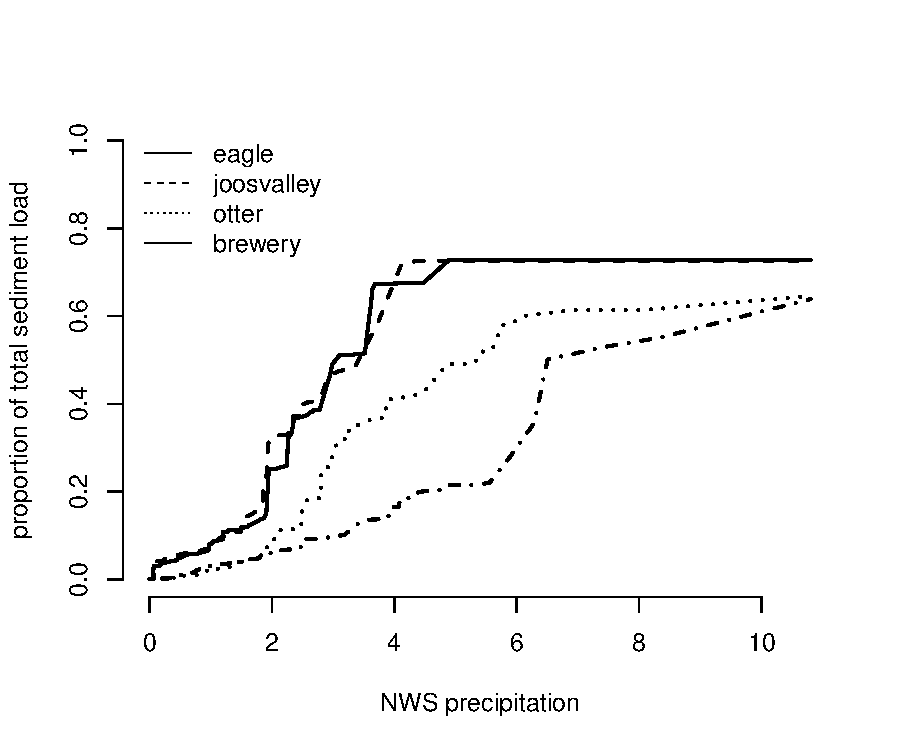
\includegraphics{loadings-figure2}
    \end{center}
    \caption{Proportion of the total sediment load contributed by rainfall events up to the size shown. Snowmelt-driven events are excluded.\label{cdf-p}}
\end{figure}

\begin{figure}
    \begin{center}
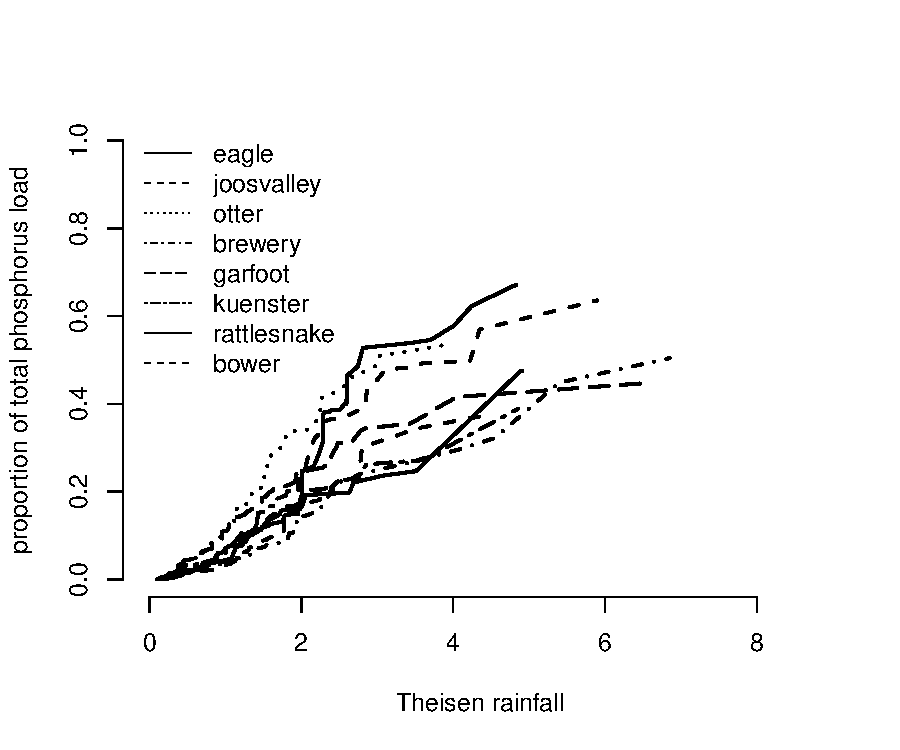
\includegraphics{loadings-figure3}
    \end{center}
    \caption{Proportion of the total phosphorus load contributed by rainfall events up to the size shown. Snowmelt-driven events are excluded.\label{cdf-s}}
\end{figure}

\begin{figure}
    \begin{center}
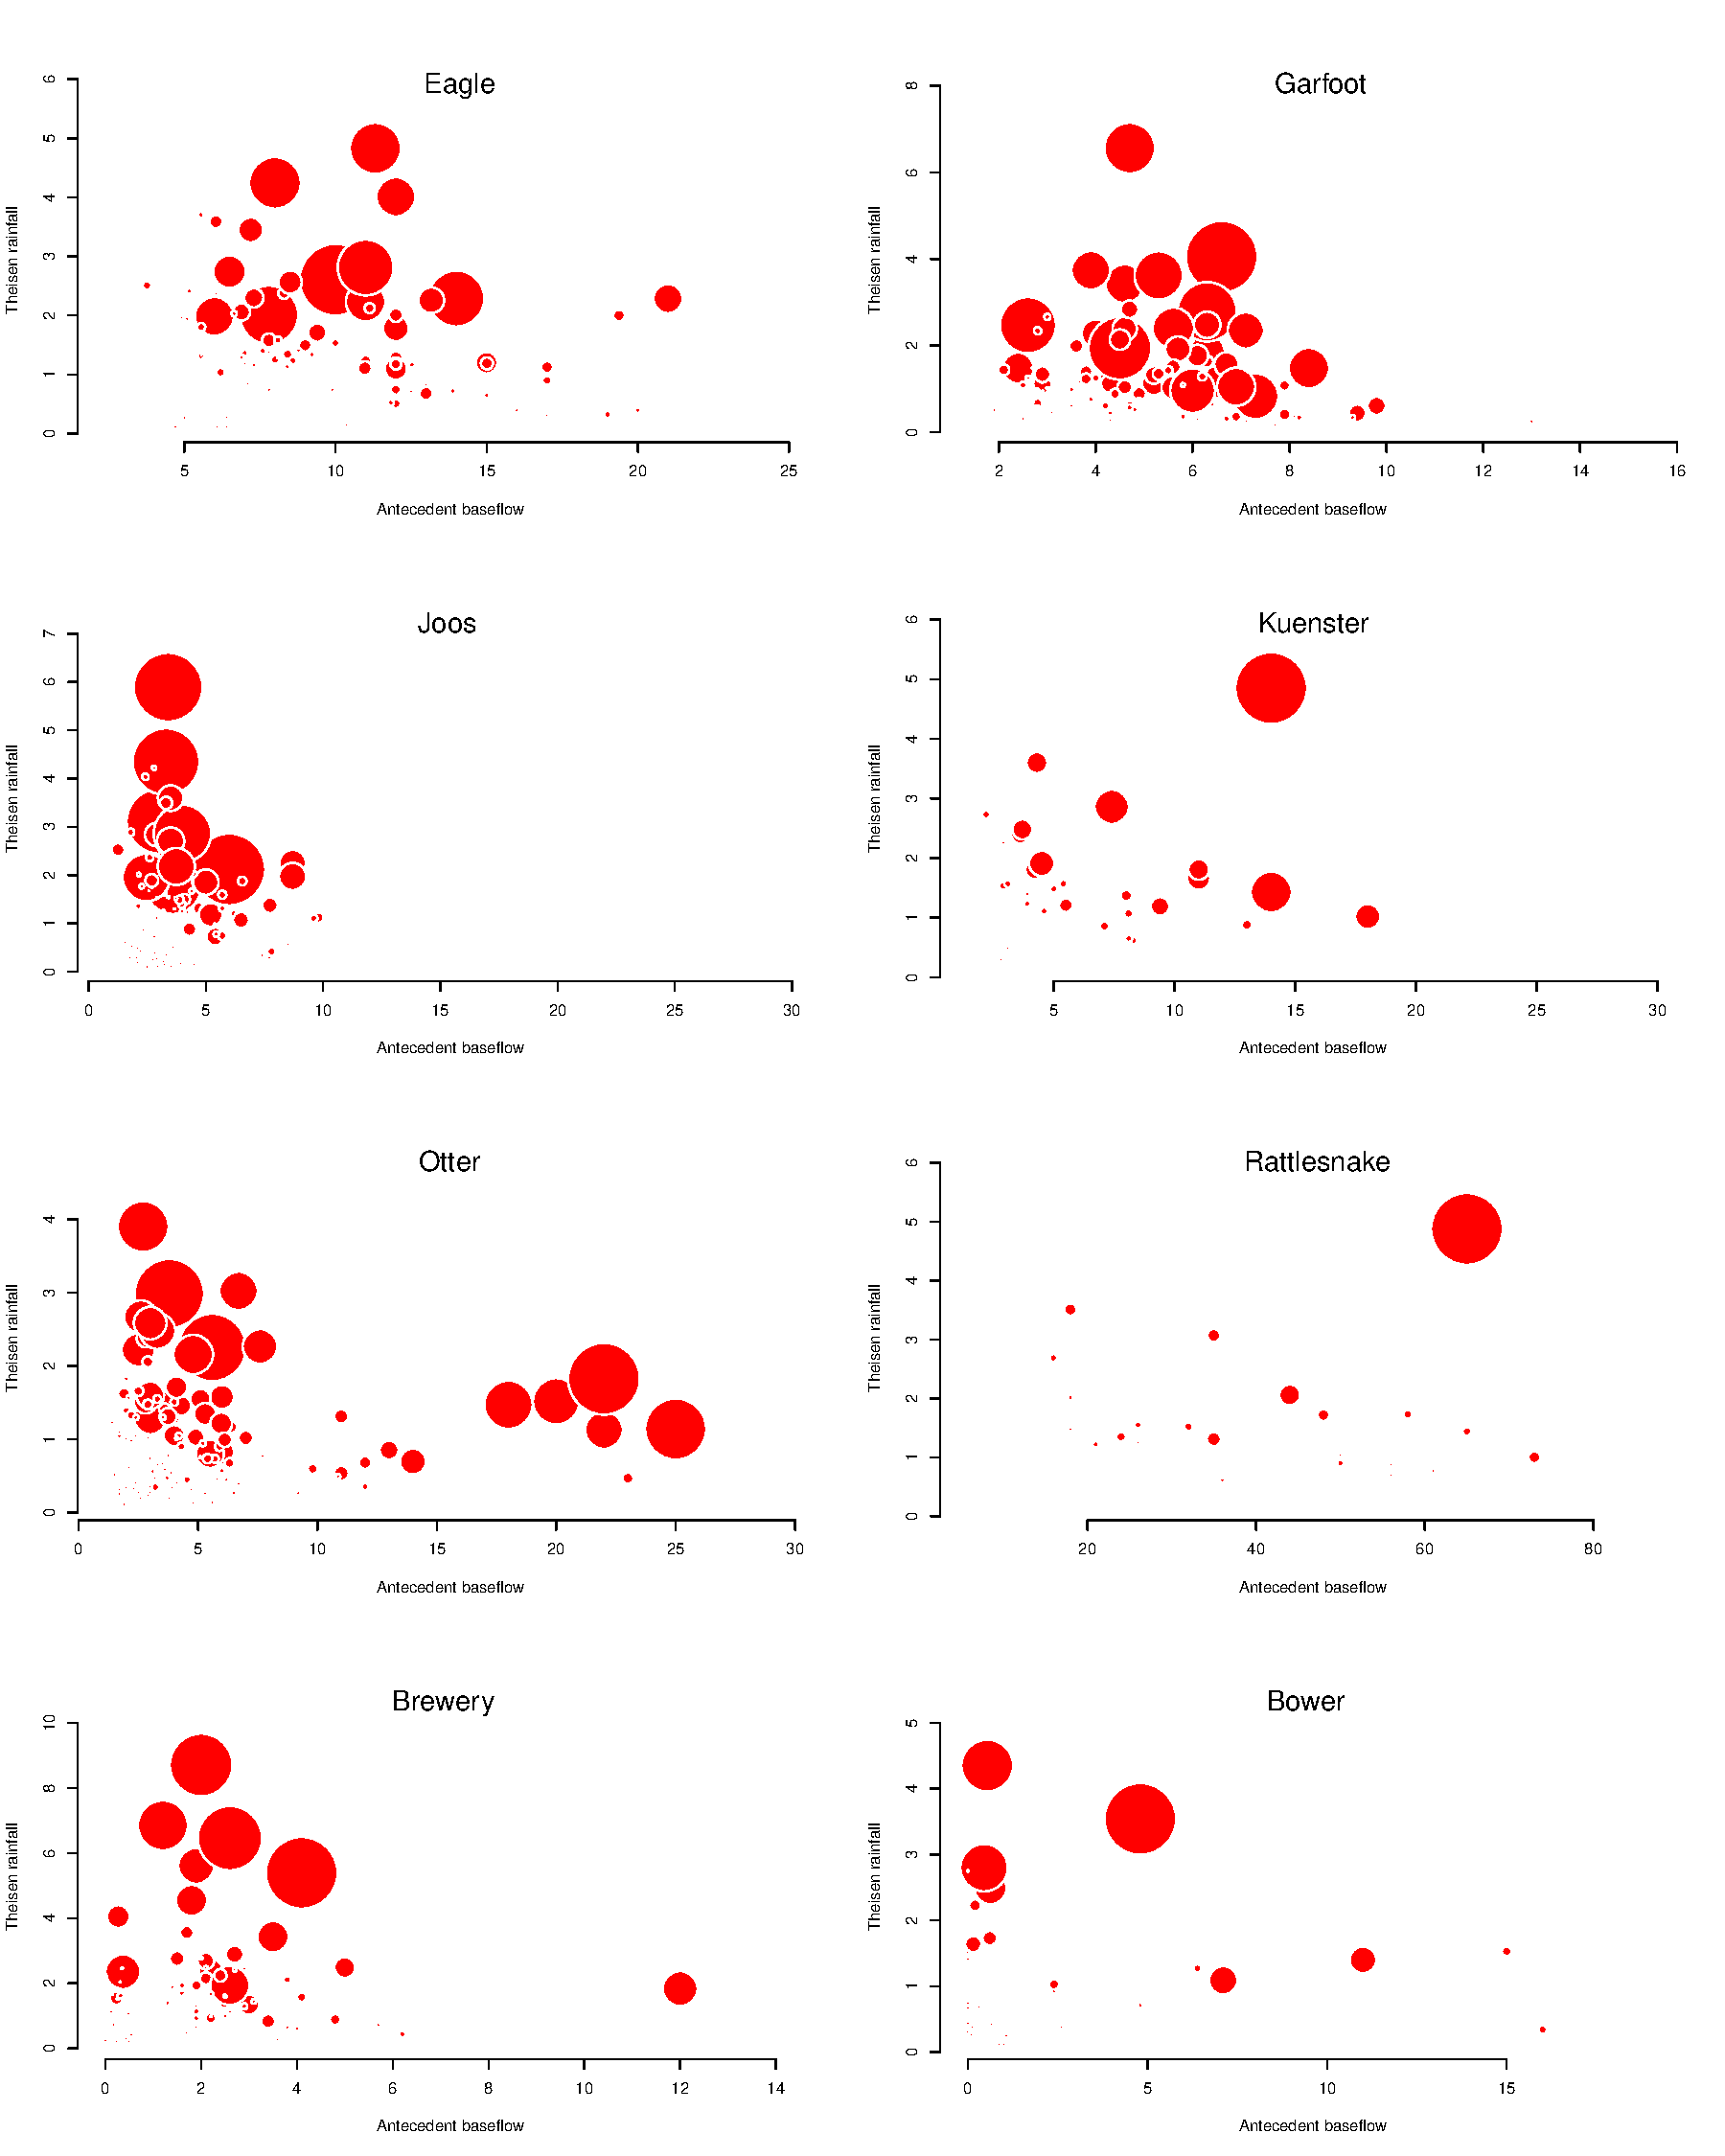
\includegraphics{loadings-figure4}
    \end{center}
    \caption{Antecedent base flow is the horizontal axis; theisen rainfall is the vertical axis. Each dot represents one event. The size of the dot shows the total sediment load contributed by that event. \label{bubbles}}
\end{figure}




\bibliographystyle{plain}
\bibliography{../../references/bibliography}

\end{document}
